\chapter{Interior-point methods}

% 11.1
\section{Inequality constrained minimization problems}
Consider a convex optimization problem with inequality constraints
\begin{align}
  \text{minimize\;\;}\quad& f_0(x)\nonumber\\
  \text{subject to}  \quad& f_i(x)\le 0,\;i=1,\dots,m\label{eq:11.1}\\
                          & Ax=b\nonumber
\end{align}
where $f_i:\R^n\rightarrow\R,\;i=0,\dots,m$ are convex and twice continuously differentiable, and $A\in\R^{p\times n}$ with $\rank A=p<n$.
We assume that
\begin{itemize}
  \item the problem is solvable, \ie an optimal $x^\ast$ exists
  \item the problem is strictly feasible, \ie there exists $x\in\D$ that satisfies
        \begin{align*}
          Ax=b,\quad f_i(x)<0,\;i=1,\dots,m
        \end{align*}
\end{itemize}

Then the Slater's constraint qualification holds, and there exists dual optimal $\lambda^\ast\in\R^m$ and $\nu^\ast\in\R^p$, together with $x^\ast$, satisfy the KKT conditions (\S\ref{subsec:5.5.3})
\begin{align}
  f_i(x^\ast)                &\le     0,\;i=1,\dots,m\nonumber\\
  Ax^\ast                    &=       b\nonumber\\
  \lambda^\ast               &\succeq 0\label{eq:11.2}\\
  \lambda_i^\ast f_i(x^\ast) &=       0,\;i=1,\dots,m\nonumber\\
  \nabla f_0(x^\ast)+\sum_{i=1}^m\lambda_i^\ast\nabla f_i(x^\ast)+A^T\nu^\ast &= 0\nonumber
\end{align}

Interior-point methods solve the problem \eqref{eq:11.1} (or the KKT conditions \eqref{eq:11.2}) by applying Newton's method to a sequence of equality constrained problems, or to a sequence of modified versions of the KKT conditions.
\subsubsection{Examples}
\textcolor{red}{\textbf{Add in the future.}}

% 11.2
\section{Logarithmic barrier function and central path}
Rewrite \eqref{eq:11.1} as an equality constrained problem
\begin{align}
  \text{minimize\;\;}\quad& f_0(x)+\sum_{i=1}^mI_\_(f_i(x))\label{eq:11.3}\\
  \text{subject to}  \quad& Ax=b\nonumber
\end{align}
where $I_\_:\R\rightarrow\R$ is the indicator function for the nonpositive reals
\begin{align*}
  I_\_(u)=
    \begin{cases}
      0,& u\le 0\\
      \infty,& u>0
    \end{cases}
\end{align*}

The problem \eqref{eq:11.3} has no inequality constraints, but the objective function is not differentiable (Newton's method cannot be applied).

% 11.2.1
\subsection{Logarithmic barrier}
Approximate the indicator function $I_\_$ by the function
\begin{align*}
  \hat{I}_\_(u)=-(1/t)\log(-u),\;\dom\hat{I}_\_=-\R_{++}
\end{align*}
where $t>0$.
The function $\hat{I}_\_$ takes on $\infty$ for $u>0$ by our convention, and then it is
\begin{itemize}
  \item convex and nondecreasing
  \item differentiable and closed
  \item the approximation becomes more accurate as $t$ increases
  \item figure \ref{fig:11.1} shows the function
\end{itemize}
\begin{figure}
  \centering
  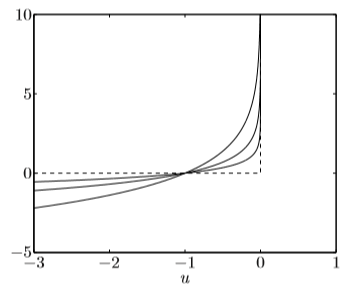
\includegraphics{fig11_1}
  \caption{The dashed lines show the function $I_\_(u)$, and the solid curves show the function $\hat{I}_\_(u)$ for $t=0.5,1,2$. The best approximation is $t=2$.}
  \label{fig:11.1}
\end{figure}
The new approximation becomes
\begin{align}
  \text{minimize\;\;}\quad& f_0(x)+\sum_{i=1}^m-(1/t)\log(-f_i(x))\label{eq:11.4}\\
  \text{subject to}  \quad& Ax=b\nonumber
\end{align}
where the objective function is convex. The \textit{logarithmic barrier} function for problem \eqref{eq:11.1} is
\begin{align}
  \phi(x)=-\sum_{i=1}^m\log(-f_i(x))\label{eq:11.5}
\end{align}
where $\dom\phi=\{x\in\R^n\mid f_i(x)<0,\;i=1,\dots,m\}$.
\begin{itemize}
  \item the quality of the approximation improves as $t$ grows
  \item if $t$ is large, the function $f_0+(1/t)\phi$ is difficult to minimize by Newton's method
  \item the above problem can be circumvented by the algorithm discussed later
\end{itemize}
The gradient and Hessian of the logarithmic barrier function $\phi$ are (\textcolor{red}{\S A.4.2 and \S A.4.4})
\begin{align*}
  \nabla\phi(x)  &= \sum_{i=1}^m\frac{1}{-f_i(x)}\nabla f_i(x)\\
  \nabla^2\phi(x)&= \sum_{i=1}^m\frac{1}{f_i(x)^2}\nabla f_i(x)\nabla f_i(x)^T+\sum_{i=1}^m\frac{1}{-f_i(x)}\nabla^2f_i(x)
\end{align*}

% 11.2.2
\subsection{Central path}
Consider the equivalent problem of \eqref{eq:11.4}
\begin{align}
  \text{minimize\;\;}\quad& tf_0(x)+\phi(x)\label{eq:11.6}\\
  \text{subject to}  \quad& Ax=b\nonumber
\end{align}

We assume \eqref{eq:11.6} can be solved via Newton's method, and it has a unique solution for each $t>0$.
Define $x^\ast(t)$ as the solution of \eqref{eq:11.6}, and the \textit{central path} associated with \eqref{eq:11.1} is defined as the set of points $x^\ast(t),\;t>0$, which we call the \textit{central points}.\par
We have the property that $x^\ast(t)$ is strictly feasible, \ie
\begin{align*}
  Ax^\ast(t)=b,\quad f_i(x^\ast(t))<0,\;i=1,\dots,m
\end{align*}
if and only if there exists a $\nu\in\R^p$ such that
\begin{align}
  0 &= t\nabla f_0(x^\ast(t))+\nabla\phi(x^\ast(t))+A^T\hat{\nu}\nonumber\\
    &= t\nabla f_0(x^\ast(t))+\sum_{i=1}^m\frac{1}{-f_i(x^\ast(t))}\nabla f_i(x^\ast(t))+A^T\hat{\nu}\label{eq:11.7}
\end{align}
which is called \textit{centrality condition}.
\begin{example}[\textit{Inequality form linear programming}]
  Consider the inequality form LP
  \begin{align}
    \text{minimize\;\;}\quad& c^Tx\nonumber\\
    \text{subject to}  \quad& Ax\preceq b\label{eq:11.8}
  \end{align}
  The logarithmic barrier function is
  \begin{align*}
    \phi(x)=-\sum_{i=1}^m\log(b_i-a_i^Tx),\;\dom\phi=\{x\mid Ax\prec b\}
  \end{align*}
  where $a_1^T,\dots,a_m^T$ are the rows of $A$. The gradien and Hessian are
  \begin{align*}
    \nabla\phi(x)=\sum_{i=1}^m\frac{1}{b_i-a_i^Tx}a_i,\quad\nabla^2\phi(x)=\sum_{i=1}^m\frac{1}{(b_i-a_i^Tx)^2}a_ia_i^T
  \end{align*}
  or, more compactly,
  \begin{align*}
    \nabla\phi(x)=A^Td,\quad\nabla^2\phi(x)=A^T\diag(d)^2A
  \end{align*}
  where $d\in\R^m,\;d_i=1/(b_i-a_i^Tx)$.
  Since $x$ is strictly feasible, we have $d\succ 0$, so Hessian is nonsingular if and only if $A$ has rank $n$.\\
  The centrality condition \eqref{eq:11.7} is
  \begin{align}
    tc+\sum_{i=1}^m\frac{1}{b_i-a_i^Tx}a_i=tc+A^Td=0\label{eq:11.9}
  \end{align}
  We have $\nabla\phi(x^\ast(t))=-tc$, \ie at a point $x^\ast(t)$ on the central path the gradient must be parallel to $-c$.
  In other words, the hyperplane $c^Tx=c^Tx^\ast(t)$ is tangent to the level set of $\phi$ through $x^\ast(t)$.
  Figure \ref{fig:11.2} shows an example with $m=6$ and $n=2$.
\end{example}
\begin{figure}
  \centering
  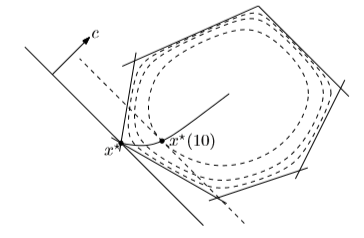
\includegraphics{fig11_2}
  \caption{The dashed curves show three contour lines of $\phi$. The line $c^Tx=c^Tx^\ast(10)$ is tangent to the contour line of $\phi$ through $x^\ast(10)$.}
  \label{fig:11.2}
\end{figure}

\subsubsection{Dual points from central path}
From \eqref{eq:11.7} we know that every central point yields a dual feasible point, and hence a lower bound of $p^\ast$.
Define
\begin{align}
  \lambda_i^\ast(t)=-\frac{1}{tf_i(x^\ast(t))},\;i=1,\dots,m,\quad\nu^\ast(t)=\frac{\hat{\nu}}{t}\label{eq:11.10}
\end{align}
we claim that the pair $\lambda^\ast(t)$, $\nu^\ast(t)$ is dual feasible.
\begin{proof}
  We have $\lambda^\ast(t)\succ 0$ since $f_i(x^\ast(t))<0$.
  The optimality conditions \eqref{eq:11.7} becomes
  \begin{align*}
    \nabla f_0(x^\ast(t))+\sum_{i=1}^m\lambda_i^\ast(t)\nabla f_i(x^\ast(t))+A^T\nu^\ast(t)=0
  \end{align*}
  we see that $x^\ast(t)$ minimizes the Lagrangian
  \begin{align*}
    L(x,\lambda,\nu)=f_0(x)+\sum_{i=1}^m\lambda_if_i(x)+\nu^T(Ax-b)
  \end{align*}
  for $\lambda=\lambda^\ast(t)$ and $\nu=\nu^\ast(t)$, which means that $\lambda^\ast(t)$, $\nu^\ast(t)$ is a dual feasible pair.
\end{proof}
The Lagrangian dual function
\begin{align*}
  g(\lambda^\ast(t),\nu^\ast(t))
    &= f_0(x^\ast(t))+\sum_{i=1}^m\lambda_i^\ast(t)f_i(x^\ast(t))+\nu^\ast(t)^T(Ax^\ast(t)-b)\\
    &= f_0(x^\ast(t))-m/t
\end{align*}
The duality gap associated with $x^\ast(t)$, $\lambda^\ast(t)$ and $\nu^\ast(t)$ is $m/t$.
An important result states
\begin{align*}
  f_0(x^\ast(t))-p^\ast\le m/t
\end{align*}
\ie $x^\ast(t)$ is no more than $m/t$-suboptimal.
This confirms the intuitive idea that $x^\ast(t)$ converges to an optimal point as $t\rightarrow\infty$.

\subsubsection{Interpretation via KKT conditions}

\subsubsection{Force field interpretation}

% 11.3
\section{The barrier method}
We know that $x^\ast(t)$ is $m/t$-suboptimal, and that a certificate of this accuracy is provided by $\lambda^\ast(t)$ and $\nu^\ast(t)$.
We take $t=m/\epsilon$ and solve the problem using Newton's method.
\begin{align*}
  \text{minimize\;\;}\quad& (m/\epsilon)f_0(x)+\phi(x)\\
  \text{subject to}  \quad& Ax=b
\end{align*}
This method could be called the \textit{unconstrained minimization method}.

% 11.3.1
\subsection{The barrier method}
A simple extension of the unconstrained minimization method does work well.
It is based on solving a sequence of unconstrained (or linearly constrained) minimization problems.
This method was first proposed by Fiacco and McCormick in the 1960s, and was called \textit{sequential unconstrained minimization technique} (SUMT).
Today the method is called the \textit{barrier method} or \textit{path-following method}.
\begin{algorithm}[\textit{Barrier method}]
  $ $\\
  \textbf{given} strictly feasible $x$, $t:=t^{(0)}$, $\mu>1$, tolerance $\epsilon>0$\\
  \textbf{repeat}
  \begin{enumerate}
    \item \textit{Centering step.} Get $x^\ast(t)$ by minimizing $tf_0+\phi$, subject to $Ax=b$, starting at $x$.
    \item \textit{Update.} $x:=x^\ast(t)$.
    \item \textit{Stopping criterion.} \textbf{quit} if $m/t<\epsilon$.
    \item \textit{Increase $t$.} $t:=\mu t$.
  \end{enumerate}
\end{algorithm}

% 11.3.2
\subsection{Examples}

% 11.3.3
\subsection{Convergence analysis}

% 11.3.4
\subsection{Newton step for modified KKT equations}

% 11.4
\section{Feasibility and phase I methods}

% 11.4.1
\subsection{Basic phase I method}

% 11.4.2
\subsection{Phase I via infeasible start Newton method}

% 11.4.3
\subsection{Examples}

% 11.5
\section{Complexity analysis via self-concordance}

% 11.5.1
\subsection{Self-concordance assumption}

% 11.5.2
\subsection{Newton iterations per centering step}

% 11.5.3
\subsection{Total number of Newton iterations}

% 11.5.4
\subsection{Feasibility problems}

% 11.5.5
\subsection{Combined phase I/phase II complexity}

% 11.5.6
\subsection{Summary}

% 11.6
\section{Problems with generalized inequalities}

% 11.6.1
\subsection{Logarithmic barrier and central path}

% 11.6.2
\subsection{Barrier method}

% 11.6.3
\subsection{Examples}

% 11.6.4
\subsection{Complexity analysis via self-concordance}

% 11.7
\section{Primal-dual interior-point methods}

% 11.7.1
\subsection{Primal-dual search direction}

% 11.7.2
\subsection{The surrogate duality gap}

% 11.7.3
\subsection{Primal-dual interior-point method}

% 11.7.4
\subsection{Examples}

% 11.8
\section{Implementation}

% 11.8.1
\subsection{Standard form linear programming}

% 11.8.2
\subsection{$\ell 1$-norm approximation}

% 11.8.3
\subsection{Semidefinite programming in inequality form}

% 11.8.4
\subsection{Network rate optimization}
